\begin{song}{title=\centering Pyšný Janek \\\normalsize Jaromír Nohavica  \vspace*{-0.3cm}}  %% sem se napíše jméno songu a autor
\moveright \stred \vbox{      %Varianta č. 1  ---> Jeden sloupec zarovnaný na střed	

\sloka 
	/: ^{G{\color{white}\_\_}}Pyšný Janku na okénku,

	pyšný v poli, ^{C\,\,\,\,\,}pyšný v ^{G\,\,\,\,\,\,\,}šenku. ^{C\,\,G} :/
	
	/: ^{D{\color{white}\_}}Kajže ty si najdeš ženku,
	
	^{D{\color{white}\_}}kajže ^{Emi}ty si ^{C{\color{white}\_\_}}najdeš ^{G}ženku. :/ Jé.

\sloka
	/: Děvuchy do kola chodí,

	za ruky se spolu vodí. :/
	
	/: Ani jedna neuškodí,
	
	ani jedna neuškodí. :/ Jé.

\sloka
	/: Bo ty, švarný, pyšný Janku,
	
	nechceš žádnů za galánku. :/
	
	/: Inum koňa, inum šklanku,

	inum koňa, inum šklanku. :/ Jé.


}
\setcounter{Slokočet}{0}
\end{song}

\begin{figure}[h]
\centering
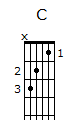
\includegraphics[width=3cm]{../Akordy/c.png}
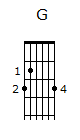
\includegraphics[width=3cm]{../Akordy/g.png}
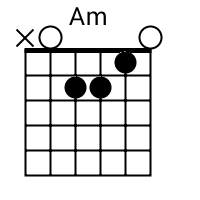
\includegraphics[width=3cm]{../Akordy/am.png}
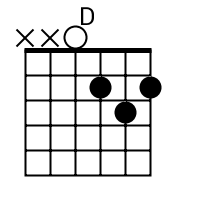
\includegraphics[width=3cm]{../Akordy/d.png}
\end{figure}
